\tocsection{\textbf{10/21/26 Lecture 24:} Triangulations, Cones, and Barycentric Subdivision}


\textbf{Recall:} An equivalent definition for $v_0, \ldots, v_n$ being in general position is that the vectors $\{v_1 - v_0, \ldots, v_n - v_0\}$ are linearly independent. In this case, the vertices form an $n$-simplex
\[ \left\{\sum_{i = 0}^{n} \lambda_iv_i \col \lambda_i \geq 0, \sum_{i = 0}^{n} \lambda_i = 1\right\} \]

Now, if $K$ is a simplicial complex, let $\abs{K}$ be the corresponding subset of $\R^n$ with the subset topology.

\begin{definition}[\textbf{Definition 24.1:} Triangulations]
    A \emph{triangulation} of a topological space $X$ is a simplicial complex $K$ and a homeomorphism from $\abs{K}$ to $X$.
\end{definition}

\begin{example}{\textbf{Example:} Triangulating $S^2$}.
    Let $X = S^2$. Then, let $\abs{K}$ be the boundary of the tetrahedron
    \fig{0.5}{Lecture24Fig1}{}
    This is homeomorphic to $S^2$.
\end{example}

If $X$ is a topological space, we had a notion of the cone
\[ CX = X \times [0, 1] / (x, 1) \sim (x', 1) \]
\fig{0.4}{Lecture24Fig2}{}

How do we do this simplicially? Let $K$ be a simplicial complex in $\R^n$. Then, consider the embedding $K \hookrightarrow \R^{n + 1}$. Then, let $v = (0, \ldots, 0, 1) \in \R^{n + 1}$. If $A$ is a simplex $(v_0, \ldots, v_k)$ in $K$, let $CA = (v_0, \ldots, v_k, v)$. Then, let
\[ CK = K \cup \{v\} \cup \{CA \col A \in K\} \]

\textbf{Example:} $n = 1$
\fig{0.45}{Lecture24Fig3}{}
Then $CK$ is a simplicial complex in $\R^{n + 1}$ and $\abs{CK}$ is homeomorphic to $C\abs{K}$.

\begin{definition}[\textbf{Definition 24.2:} Isomorphisms of Simplicial Complexes]
    Let $K, L$ be simplicial complexes, possibly in different Euclidean spaces. An \emph{isomorphism} between $K$ and $L$ is a bijection $\phi : \{\tt{vertices in } K\} \to \{\tt{vertices in } L\}$, so $(v_0, \ldots, v_k)$ is a simplex in $K$ iff $(\phi v_0, \ldots, \phi v_k)$ is a simplex in $L$.
\end{definition}


\textbf{Fact:} If the above holds, $\abs{K}$ and $\abs{L}$ are homeomorphic, since $\phi$ can be defined as a linear map.

\begin{definition}[\textbf{Definition 24.3:} Interiors of Simplices].
    If $K$ is a simplex in $\R^n$ with vertices $(v_0, \ldots, v_k)$, then the \emph{interior} is
    \[ \tt{int}(K) = \left\{\sum_{i = 0}^{k} \lambda_iv_i \col \lambda_i > 0, \sum_{i = 0}^{k} \lambda_i = 1\right\} \]
\end{definition}

\begin{lemma}[\textbf{Proposition 24.4}]
    Suppose $K$ is a finite simplicial complex in $\R^n$.
    \begin{enumerate}
        \item $\abs{K}$ is compact.
        \item Each point in $\abs{K}$ lies in the interior of a unique simplex.
        \item The closed subsets of $\abs{K}$ are those that intersect each simplex in a closed subset.
        \item If $\abs{K}$ is connected, it is path connected.
    \end{enumerate}
\end{lemma}
\begin{proof}{Proof:}
    \textbf{1)} Since each simplex is closed and bounded in $\R^n$, and as $\abs{K}$ is a finite union of these, it is compact.\\

    \textbf{2)} First, we want to show that each $x$ in $\abs{K}$ is in the interior of some simplex.\\

    First, $x$ must be in some simplex $(v_0, \ldots, v_k)$ in $K$. Then, write
    \[ x = \sum_{i = 0}^{k} \lambda_iv_i, \quad \lambda_i \geq 0,\ \sum \lambda_i = 1 \]
    Then, $x$ must be in the interior of the simplex spanned by the vertices for which $\lambda_i > 0$ (at least one must exist).\\

    To show this is unique, suppose $x \in \tt{int}(A) \cap \tt{int}(B)$, so $x \in A \cap B$, so $x$ must lie in a common face of both $A$ and $B$. However, if $x$ is in the interior of $A$, all of its weights corresponding to the vertices of $A$ must be positive, so the face must be $A$. Similarly, the face must be $B$, so $A = B$.\\

    \textbf{3)} $(\Rightarrow)$ If $C \subseteq \abs{K}$ is closed, then as each simplex is closed, the intersection of $C$ with any simplex is itself closed in $\abs{K}$.\\

    $(\Leftarrow)$ Suppose $C \subseteq \abs{K}$ and $C \cap A$ is closed for all simplices $A \in K$. Then, $C \cap A = A \cap D$ for some closed $D$ in $\abs{K}$. Since $A$ is closed, we see that $C \cap A$ is closed in $\abs{K}$. Thus, as
    \[ C = \bigcup_{A \in K} C \cap A \]
    is a finite union of closed sets, it is closed.\\

    \textbf{4)} Given an $x \in \abs{K}$, for some $\delta > 0$, $B(x, \delta) \cap \abs{K}$ is path connected. Hence, $\abs{K}$ is locally path connected, so as $\abs{K}$ is connected, $\abs{K}$ is path connected.

    $\qed$
\end{proof}

\begin{definition}[\textbf{Definition 24.5:} Barycenters]
    If $A \subseteq \R^n$ is a simplex with vertices $v_0, \ldots, v_k$, then its \emph{barycenter} is
    \[ \widehat{A} = \frac{1}{k + 1}\sum_{i = 0}^{k} v_i \in A \]
\end{definition}

If $K$ is a simplicial complex, then we will define its \emph{barycentric subdivision} $K'$ as follows:
\fig{0.45}{Lecture24Fig4}{}

Let's formalize this.\\


\textbf{Notation:} If $A$ is a proper face of $B$, write $A < B$.

\begin{definition}[\textbf{Definition 24.6:} Barycentric Subdivision]
    If $A_0 < \cdots < A_k$ is an increasing sequence of simplices in $K$, then
    \[ (\widehat{A}_0, \widehat{A}_1, \ldots, \widehat{A}_k) \]
    are the vertices of a $k$-simplex in $K'$.
\end{definition}

\textbf{Example:} If
\begin{center}
    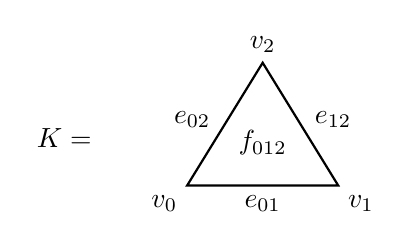
\begin{tikzpicture}[scale = 1.2]
        \node at (-1.3, 0.5) {$K =$};
        \draw[thick] (0, 0) -- (1.6, 0) -- (0.8, 1.3) -- cycle;
        \node[below left] at (0, 0) {$v_0$};
        \node[below right] at (1.6, 0) {$v_1$};
        \node[above] at (0.8, 1.3) {$v_2$};
        \node[below] at (0.8, 0) {$e_{01}$};
        \node[right] at (1.25, 0.7) {$e_{12}$};
        \node[left] at (0.35, 0.7) {$e_{02}$};
        \node at (0.8, 0.45) {$f_{012}$};
    \end{tikzpicture}
\end{center}
then $K'$ consists of
\begin{itemize}
    \item \underline{$0$-simplices:} $\{\widehat{v}_0, \widehat{v}_1, \widehat{v}_2, \widehat{e}_{01}, \widehat{e}_{12}, \widehat{e}_{02}, \widehat{f}_{012}\}$
    \item[\textcolor{red}{$\bullet$}] \underline{$1$-simplices:}
    \begin{align*}
        \{&(\widehat{v}_0, \widehat{e}_{01}), (\widehat{v}_0, \widehat{e}_{02}), (\widehat{v}_0, \widehat{f}_{012}),\\
        &(\widehat{v}_1, \widehat{e}_{01}), (\widehat{v}_1, \widehat{e}_{12}), (\widehat{v}_1, \widehat{f}_{012}),\\
        &(\widehat{v}_2, \widehat{e}_{12}), (\widehat{v}_2, \widehat{e}_{02}), (\widehat{v}_2, \widehat{f}_{012}),\\
        &(\widehat{e}_{01}, \widehat{f}_{012}), (\widehat{e}_{12}, \widehat{f}_{012}), (\widehat{e}_{02}, \widehat{f}_{012})\}
    \end{align*}
    \item[\textcolor{blue}{$\bullet$}] \underline{$2$-simplices:}
    \begin{align*}
        \{&(\widehat{v}_0, \widehat{e}_{01}, \widehat{f}_{012}), (\widehat{v}_0, \widehat{e}_{02}, \widehat{f}_{012}),\\
        &(\widehat{v}_1, \widehat{e}_{01}, \widehat{f}_{012}), (\widehat{v}_1, \widehat{e}_{12}, \widehat{f}_{012}),\\
        &(\widehat{v}_2, \widehat{e}_{12}, \widehat{f}_{012}), (\widehat{v}_2, \widehat{e}_{02}, \widehat{f}_{012})\}
    \end{align*}
\end{itemize}
so
\begin{center}
    $K' = $ \raisebox{-0.45\height}{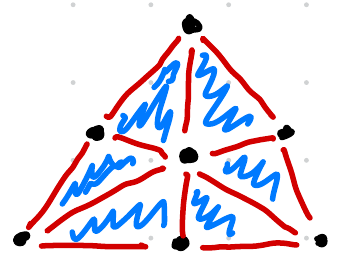
\includegraphics[scale = 0.5]{Lecture24Fig5}}
\end{center}
